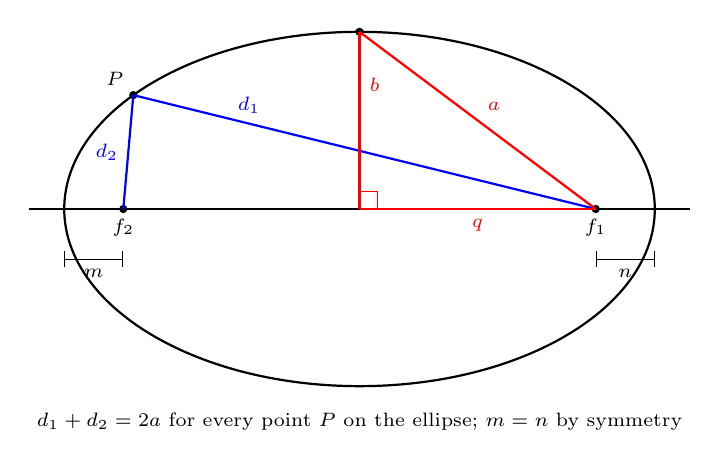
\begin{tikzpicture}[scale=0.75, every node/.style={font=\scriptsize}]
  \draw (-5.6,0) -- (5.6,0);
  \draw[thick] (0,0) ellipse (5 and 3);
  \coordinate (F1) at (4,0);
  \coordinate (F2) at (-4,0);
  \coordinate (P) at ({5*cos(140)},{3*sin(140)});
  \coordinate (T) at (0,3);
  \fill (F1) circle (2pt) node[below] {$f_1$};
  \fill (F2) circle (2pt) node[below] {$f_2$};
  \fill (P) circle (2pt) node[above left] {$P$};
  \draw[blue, thick] (P) -- (F1) node[pos=0.25, above] {$d_1$};
  \draw[blue, thick] (P) -- (F2) node[midway, left] {$d_2$};
  \fill (T) circle (2pt);
  \draw[red, thick] (F1) -- (T) node[midway, above right] {$a$};
  \draw[red, thick] (0,0) -- (T) node[pos=0.7, right] {$b$};
  \draw[red, thick] (0,0) -- (F1) node[midway, below] {$q$};
  \draw[red] (0.3,0) -- (0.3,0.3) -- (0,0.3);
  \draw[{Bar[]}-{Bar[]}] (4,-0.85) -- (5,-0.85) node[midway, below] {$n$};
  \draw[{Bar[]}-{Bar[]}] (-5,-0.85) -- (-4,-0.85) node[midway, below] {$m$};
  \node at (0,-3.6) {$d_1+d_2=2a$ for every point $P$ on the ellipse; $m=n$ by symmetry};
\end{tikzpicture}
